\chapter{Anexos}
        
    \section{Anexo I. Análisis de campo}
    
        \subsection{Encuesta}
            Las siguientes preguntas hacen referencia a los procesos para realizar trámites del ámbito de la gestión educativa de la Escuela Superior de Cómputo.
    
            \begin{multicols}{2}
        
                \begin{enumerate}
                    \item ¿Cómo te enteras del procedimiento para llevar a cabo tus trámites?
                    \begin{enumerate}[(a)]
                        \item Compañeros o Amigos
                        \item Página web de la escuela
                        \item Redes sociales
                        \item Semana de inducción
                        \item Atención en ventanilla
                        \item Atención telefónica 
                        \item Otro
                    \end{enumerate}
                
                    \item ¿Has tenido problemas a la hora de realizar algún trámite?
                    \begin{enumerate}[(a)]
                        \item SI
                        \item No
                    \end{enumerate}
                    \item Si la respuesta fue sí, ¿Cuáles consideras que son los 3 principales impedimentos a la hora de realizar un trámite?
                    \begin{enumerate}[(a)]
                        \item Falta de información
                        \item Falta de claridad en el proceso
                        \item Falta de documentación
                        \item Información no actualizada 
                        \item Fuera de tiempo
                        \item Otro
                    \end{enumerate}
                    \item ¿Requeriste más de un medio para poder obtener la información que necesitabas?
                    \begin{enumerate}[(a)]
                        \item SI
                        \item No
                    \end{enumerate}
                    \item ¿Alguna vez has intentado pedir asesoría para realizar un trámite por medio de internet?
                    \begin{enumerate}[(a)]
                        \item SI
                        \item No
                    \end{enumerate}
                    Si la respuesta fue sí, contesta las preguntas 6-9: 
                    \item ¿En qué medio buscaste la asesoría?
                    \begin{enumerate}[(a)]
                        \item Página de facebook
                        \item Messenger de facebook
                        \item Twitter
                        \item Correo electrónico
                        \item Otro
                    \end{enumerate}
                
                    \item ¿En cuanto tiempo te obtuviste la asesoría?
                    \begin{enumerate}[(a)]
                        \item En menos de una hora
                        \item Ese mismo día más tarde
                        \item Días después
                        \item No obtuve una respuesta
                    \end{enumerate}
                
                    \item La información que te proveyeron fue: (Marca las necesarias)
                    \begin{enumerate}[(a)]
                        \item Completa
                        \item Oportuna
                        \item Relevante
                        \item Accesible
                        \item Entendible
                        \item Clara
                        \item Precisa
                        \item Satisfactoria
                    \end{enumerate}
                
                    \item ¿Como fue la experiencia a la hora de solicitar la información?
                    \begin{enumerate}[(a)]
                        \item Muy satisfactoria 
                        \item Buena
                        \item Regular
                        \item Mala
                    \end{enumerate}
                    \item Si las respuestas a través de Facebook Messenger a tus dudas sobre distintos trámites fueran contestadas con prontitud. ¿Qué prioridad de uso le darías a este servicio?
                    \begin{enumerate}[(a)]
                        \item Seria mi primera opción
                        \item Estaría entre mis opciones
                        \item No lo usaría
                    \end{enumerate}
                \end{enumerate}
                
        \end{multicols}
    
        La propuesta de solución a este problema es la creación de un prototipo de agente conversacional popularmente conocido como chatbot proveído a través del aplicativo de facebook para mensajería instantánea “Messenger”, este estará enfocado a la resolución de preguntas frecuentes formuladas por el alumnado de ESCOM.
        
        
        La información recabada en esta encuesta nos será de gran utilidad, por parte de los integrantes y directores del trabajo terminal 2019-A087 le damos las gracias por completar esta encuesta.
    
        \subsection{Resultados}
            \begin{figure}[H]
                \centering
                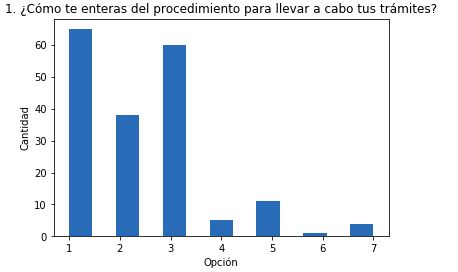
\includegraphics[width=.8\linewidth]{Latex/Classes/Imagenes/1.png}
                \caption{Gráfico de barras: Pregunta 1}
            \end{figure}
            \begin{figure}[H]
                \centering
                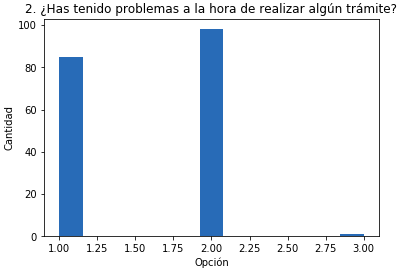
\includegraphics[width=.8\linewidth]{Latex/Classes/Imagenes/2.png}
                \caption{Gráfico de barras: Pregunta 2}
            \end{figure}
            \begin{figure}[H]
                \centering
                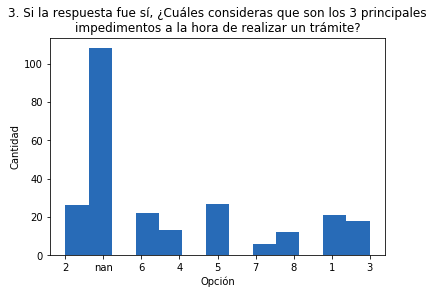
\includegraphics[width=.8\linewidth]{Latex/Classes/Imagenes/3.png}
                \caption{Gráfico de barras: Pregunta 3}
            \end{figure}
            \begin{figure}[H]
                \centering
                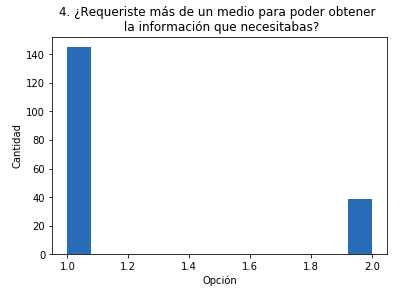
\includegraphics[width=.8\linewidth]{Latex/Classes/Imagenes/4.png}
                \caption{Gráfico de barras: Pregunta 4}
            \end{figure}
            \begin{figure}[H]
                \centering
                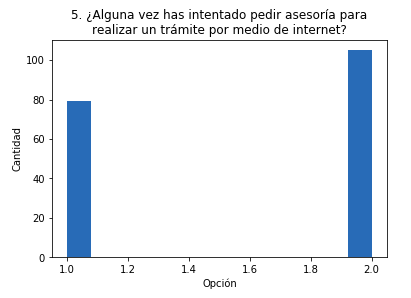
\includegraphics[width=.8\linewidth]{Latex/Classes/Imagenes/5.png}
                \caption{Gráfico de barras: Pregunta 5}
            \end{figure}
            \begin{figure}[H]
                \centering
                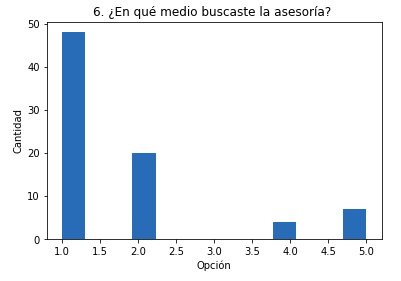
\includegraphics[width=.8\linewidth]{Latex/Classes/Imagenes/6.png}
                \caption{Gráfico de barras: Pregunta 6}
            \end{figure}
            \begin{figure}[H]
                \centering
                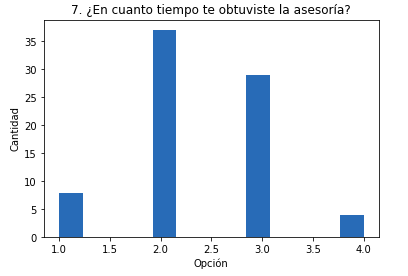
\includegraphics[width=.8\linewidth]{Latex/Classes/Imagenes/7.png}
                \caption{Gráfico de barras: Pregunta 7}
            \end{figure}
            \begin{figure}[H]
                \centering
                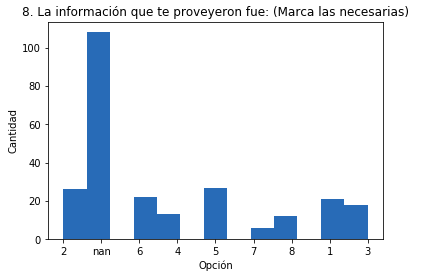
\includegraphics[width=.8\linewidth]{Latex/Classes/Imagenes/8.png}
                \caption{Gráfico de barras: Pregunta 8}
            \end{figure}\begin{figure}[H]
                \centering
                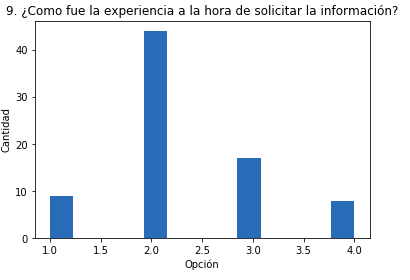
\includegraphics[width=.8\linewidth]{Latex/Classes/Imagenes/9.png}
                \caption{Gráfico de barras: Pregunta 9}
            \end{figure}
            \begin{figure}[H]
                \centering
                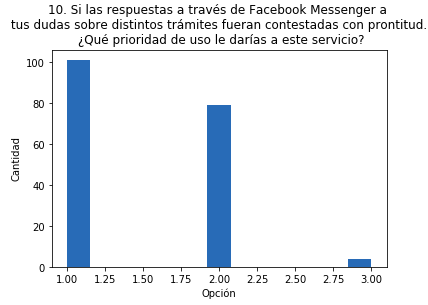
\includegraphics[width=.8\linewidth]{Latex/Classes/Imagenes/10.png}
                \caption{Gráfico de barras: Pregunta 10}
            \end{figure}
            
            \begin{figure}[H]
                \centering
                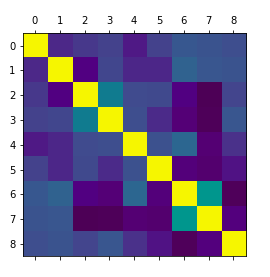
\includegraphics[width=.5\linewidth]{Latex/Classes/Imagenes/correlacion.png}
                \caption{Mapa de correlación de variables ente las preguntas de la encuesta}
            \end{figure}
    
    \newpage
    \section{Anexo II. Entrevista }
    \section{Anexo III. Métricas del ajuste de la completitud técnica}
        \begin{enumerate}
            \item Comunicación de Datos
                \begin{description}
                    \item[0:] Aplicación es batch exclusivamente
                    \item[1-2] Impresión o entrada de datos remota
                    \item[3-5] Teleproceso (TP) interactivo
                    \item[3] TP interface a un proceso batch
                    \item[5] La aplicación se interactiva
                \end{description}
            \item Función Distribuída. "Distribuída" significa que los componentes de la aplicación están distribuídos en dos o más procesadores diferentes.
                \begin{description}
                    \item[0:] La aplicación no ayuda a la trasferencia de datos o a la función de procesamiento entre los componentes del sistema
                    \item[1] La aplicación prepara datos para el usuario final de otro procesador
                    \item[2-3] Los datos se preparan para trasferencia, se trasfieren y se procesan en otro componente del sistema
                    \item[4] Igual que 2-3, pero con realimentación al sistema inicial
                    \item[5] Las funciones de procesamiento se realizan dinámicamente en el componente más apropiado del sistema.
                \end{description}
            \item Rendimiento (referido a la importancia de respuesta dentro de todo el sistema)
                \begin{description}
                    \item[0, 3:]Análisis y diseño de las consideraciones del rendimiento son estándar. No se requieren requerimientos especiales por parte del usuario
                    \item[4:]En la fase de diseño se incluyen tareas del análisis del rendimiento para cumplir los requerimientos del usuario
                    \item[5:]Además se utilizan herramientas de análisis del rendimiento en el diseño, desarrollo e instalación
                \end{description}
            \item Configuración utilizada masivamente (referente a la importancia del entorno)
                \begin{description}
                    \item[0, 3:]La aplicación corre en una máquina estándar sin restricciones de operación
                    \item[4:]Restricciones de operación requieren características específicas de la aplicación en el procesador central
                    \item[5:]Además hay restricciones específicas a la aplicación en los componentes distribuídos del sistema.
                \end{description}
            \item Tasas de Transacción (una alta llegada de transacciones provoca problemas más allá de los de la característica 3)
                \begin{description}
                    \item[0, 3:]Las tasas son tales que las consideraciones de análisis de rendimiento son estándares
                    \item[4:]En la fase de diseño se incluyen tareas de análisis de rendimiento para verificar las altas tasas de transacciones
                    \item[5:]Además se utilizan herramientas de análisis del rendimiento.
                \end{description}
            \item Entrada On-Line de datos
                \begin{description}
                    \item[0, 2:]Hasta el 15\% de las transacciones tienen entrada interactiva
                    \item[3, 4:]15\% al 30\% tienen entrada interactiva
                    \item[5:]30\% al 50\% tienen entrada interactiva.
                \end{description}
            \item Diseño para la eficiencia de usuario final
                \begin{description}
                    \item[0:]Sistema batch
                    \item[1, 3:]No se especifican requerimientos especiales
                    \item[4:]Se incluyen tareas de diseño para la consideración de factores humanos
                    \item[5:]Además se utilizan herramientas especiales o de prototipado para promover la eficiencia.
                \end{description}
            \item Actualización On-Line
                \begin{description}
                    \item[0:]Nada
                    \item[1, 2:]Actualización on line de los ficheros de control. El volumen de actualización es bajo y la recuperación fácil.
                    \item[3:]Actualización on line de la mayoría de los ficheros internos lógicos
                    \item[4:]Además es esencial la protección contra la pérdida de datos
                    \item[5:]Además se considera el coste de recuperación de volúmenes elevados.
                \end{description}
            \item Complejidad del procesamiento (esto es complejidad interna más allá de las convenciones de cuenta de entidades de MkII FPA).
                ¿Qué características tiene la aplicación?
                \begin{itemize}
                    \item mucho procesamiento matemático y/o lógico
                    \item muchas excepciones de procesamiento, muchas transacciones incompletas y mucho reprocesamiento de las transacciones
                    \item procesamiento de seguridad y/o control sensitivo
                \end{itemize}
                \begin{description}
                    \item[0:]No se aplica nada de esto
                    \item[1, 3:]Se aplica alguna cosa
                    \item[4:]Se aplican dos cosas
                    \item[5:]Se aplica todo.
                \end{description}
            \item Utilizable en otras aplicaciones (el código se diseña para que sea compartido o utilizable por otras aplicaciones  -no confundir con 13).
                \begin{description}
                    \item[0, 1:]Una aplicación local que responde a las necesidades de una organización usuaria
                    \item[2, 3:]La aplicación utiliza o produce módulos comunes que consideran más necesidades que las del usuario
                    \item[4, 5:]Además, la aplicación se empaquetó y documentó con el propósito de fácil reutilización
                \end{description}
            \item Facilidad de Instalación
                \begin{description}
                   \item[0, 1:]No se requieren por parte del usuario facilidades especiales de conversión e instalación
                   \item[2, 3:]Los requerimientos de conversión e instalación fueron descritos por el usuario y se proporcionaron guías de conversión e instalación
                   \item[4, 5:]Además se proporcionaron y probaron herramientas de conversión e instalación
                \end{description}
            \item Facilidad de Operación
                \begin{description}
                   \item[0:]No se especifican por parte del usuario consideraciones específicas de operación
                   \item[1, 2:]Se requieren, proporcionan y prueban procesos específicos de arranque, backup y recuperación
                   \item[3, 4:]Además la aplicación minimiza la necesidad de actividades manuales, tales como instalación de cintas y papel
                   \item[5:]La aplicación se diseña para operación sin atención
                \end{description}
            \item Puestos Múltiples. Añadir puntos por cada uno de los siguientes factores
                \begin{description}
                   \item[0:]El usuario no requiere la consideración de más de un puesto
                   \item[1:]De uno a cuatro puestos
                   \item[2:]Cinco o más puestos
                   \item[1:]Se proporciona documentación y plan de apoyo para soportar la aplicación en varios lugares
                   \item[2:]Los puestos están en países diferentes
                \end{description}
            \item Facilidad de Cambio (esfuerzo específico de diseño para facilitar cambios futuros). Añadir puntos por cada uno de los siguientes factores
                \begin{description}
                   \item[0:]No hay requerimientos especiales del usuario para minimizar o facilitar el cambio
                   \item[1, 3:]Se proporciona capacidad de consulta flexible
                   \item[4, 5:]Datos importantes de control se mantienen en tablas que son actualizadas por el usuario a través de procesos on-line interactivos.
                \end{description}
            \item Requerimientos de otras Aplicaciones
                \begin{description}
                   \item[0:]El sistema es stand-alone
                   \item[1, 4:]Requerimientos del sistema para interfaces o compartición de datos deben ser sincronizados con otras aplicaciones
                   \item[5:]Se deben sincronizar los requerimientos del sistema con cuatro o más aplicaciones
                \end{description}
            \item Seguridad, Privacidad y Auditoría. Añadir puntos por cada uno de los siguientes factores
                \begin{description}
                   \item[1:]Si el sistema debe cumplir requerimientos personales (incluso legales) de privacidad
                   \item[1:]Si el sistema debe cumplir requerimientos especiales de auditoría
                   \item[1, 2:]Si el sistema debe cumplir requerimientos excepcionales de seguridad para prevenir pérdidas de naturaleza financiera o militar
                   \item[1:]Si se requiere el criptográfico de los datos de las comunicaciones
                 \end{description}
            \item Necesidad de Adiestramiento al Usuario
                \begin{description}
                   \item[0:]Si no es necesario material ni cursos
                   \item[1, 4:]Si se requiere entrenamiento especial o se proporcionan facilidades de ayuda on-line
                   \item[5:]Se requiere un sistema separado de entrenamiento o simulador
                \end{description}
    
            \item Uso directo de otras empresas
                \begin{description}
                   \item[0:]No existe otra empresa conectada al sistema
                   \item[1:]Los datos se envían o reciben de empresas conocidas
                   \item[2:]Empresas conocidas están conectadas al sistema en modo de lectura solamente
                   \item[3, 4:]Empresas conocidas están conectadas directamente al sistema con capacidad de actualización on-line
                   \item[5:]Empresas desconocidas (público en general o un grupo demasiado extenso como para ser adiestrado) pueden acceder al sistema
                \end{description}
            \item Documentación. Contar 1 por cada tipo de documento listado a continuación que se entrega al final del proyecto.
                \begin{itemize}
                    \item Especificación Funcional del Sistema (datos y procesos)
                    \item Especificación Técnica del Sistema
                    \item Documentación del programa (al menos diagramas de flujo)
                    \item Librería de Elementos de Datos
                    \item Elemento de Datos/ Registro/ X-referencia del programa
                    \item Manual de usuario
                    \item Folleto de información general del sistema
                    \item Librería de datos de prueba
                    \item Material de curso de adiestramiento al usuario
                    \item Documentos de coste/beneficio del sistema
                    \item Informe de petición de cambios y errores
                \end{itemize}
                Se calcula el grado de influencia utilizando la siguiente tabla
                \begin{enumerate}
                   \item si 0-2 tipos de documento
                   \item si 3-4
                   \item si 5-6
                   \item si 7-8
                   \item si 9-10
                   \item si 11-12 tipos de documento
                \end{enumerate}
        \end{enumerate}
    
    
